\chapter{Modify your agent code}

This section is to help you get started hacking your own version of the \textsc{Becca} agent. It's still very new, and there's a lot of room for improvement, so don't be afraid to jump in and start rewiring it.

\section{How is the agent code structured?}

This section will give just an overview of the structure so that you have some idea about where to start making changes. The overall structure of \textsc{Becca} is shown in Figure~\ref{becca_block}. A thorough description is included in Appendices~\ref{perceiver_chapter} and~\ref{actor_chapter}. 

\begin{figure}
\centering
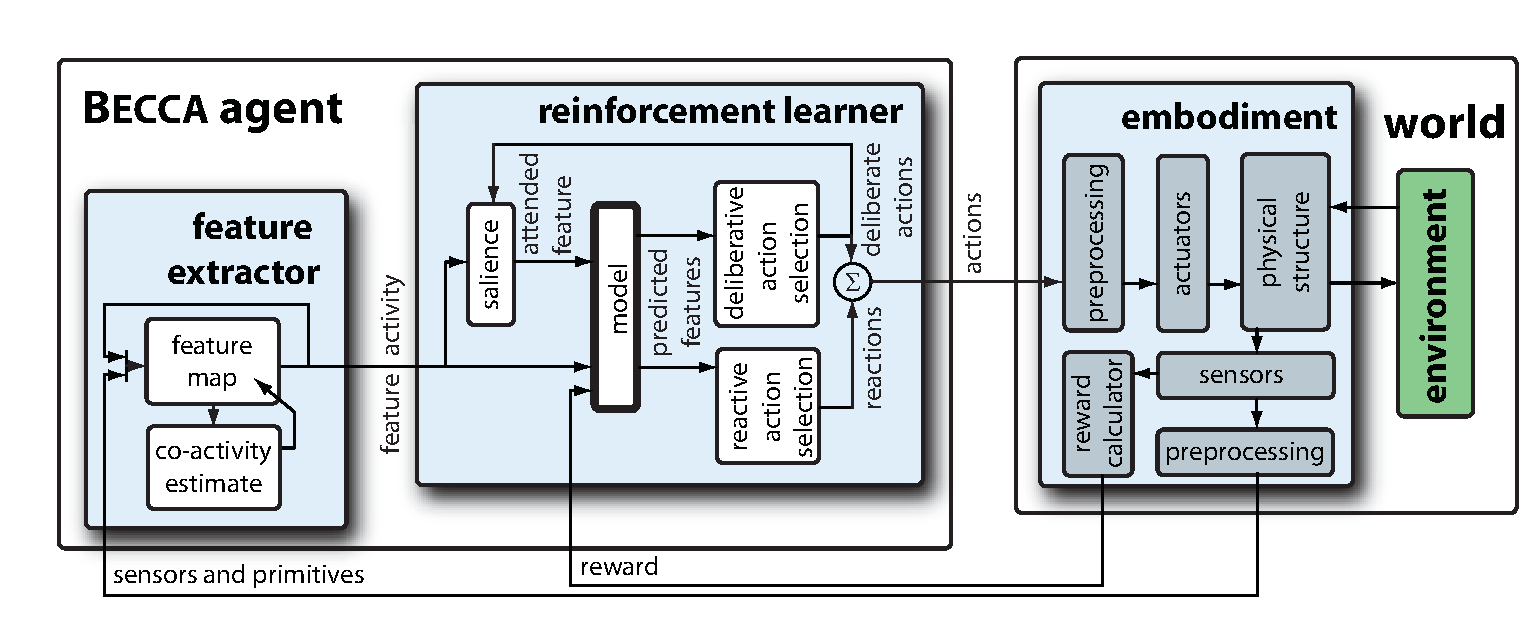
\includegraphics[height=6cm]{figs/becca_0.4.3_block.eps}
\caption{A high-level block diagram of how \textsc{Becca} is put together.}
\label{becca_block}
\end{figure}

Figure~\ref{class_structure} shows the major classes. In the code, each class is contained in a module with a lowercase version of the same name. A brief description of the major functions of each class is given below.

\begin{figure}
\centering
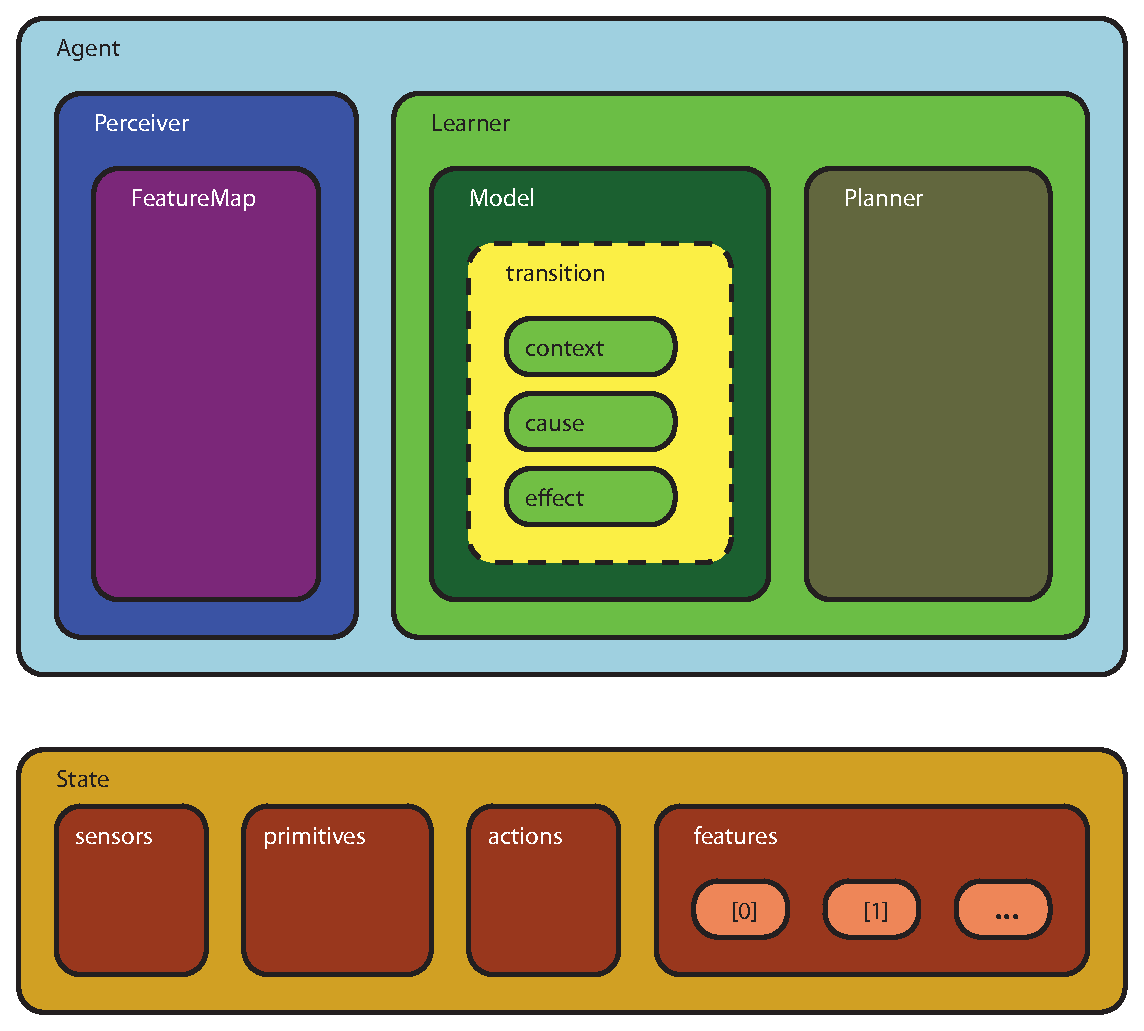
\includegraphics[height=6cm]{figs/class_structure.eps}
\caption{The class structure of \textsc{Becca}'s agent code.}
\label{class_structure}
\end{figure}

\subsection{\texttt{state}}
Represents the activity of primitives, features, and actions at a point in time. Although this was a separate class in earlier versions, numpy arrays were found to be adequate for containing state. Using them simplified the code and sped up computation.

\subsection{\texttt{Agent}}
\begin{itemize}
\item Performs executive functions, such as saving and reporting.
\item Calls \texttt{Perceiver.step()} and  \texttt{Actor.step()} at each time step.
\end{itemize}

\subsection{\texttt{Perceiver}}
\begin{itemize}
\item Forms inputs into features.
\item Determines which features are active at each time step.
\item Feeds those features back as additional inputs.
\end{itemize}

\subsection{\texttt{Actor}}
\begin{itemize}
\item Chooses which feature to attend to.
\item Calls \texttt{Model.step()} and  \texttt{Planner.step()} at each time step.
\end{itemize}

\subsection{\texttt{Model}}
\begin{itemize}
\item Contains a library of \texttt{transition}s, each consisting of four states: a \texttt{context}, a \texttt{cause}, an \texttt{effect}, and an \texttt{effect\_uncertainty}.  \texttt{transition}s are conceptual only, and are not actually member variables.
\item Finds similar transitions in a library.
\item Records new transitions in the library.
\item Updates transitions in the library.
\end{itemize}

\subsection{\texttt{Planner}}
\begin{itemize}
\item Based on the \texttt{Agent}'s current state and history, chooses an action likely to bring reward.
\item Refers to the \texttt{Model} in order to make predictions.
\end{itemize}

\subsection{Utility modules: \texttt{utils} and \texttt{viz\_utils}}
\begin{itemize}
\item Performs general math chores. May be used by multiple classes.
\item Visualizes the internal states of classes for the user.
\end{itemize}

\subsection{TCP/IP communication implementation: \texttt{server.py}}
SeH wrote this module, creating a TCP/IP interface to the \textsc{Becca} agent. It allows you to hook up a simulation or physical robot world that is speaking something other than Python. This extension enlarges the set of things that \textsc{Becca} can talk to a great deal.

\section{Is my agent better than the core agent?}
The most natural question to ask after changing the agent is whether the new version is better than the old one.\footnote{This is also a natural question to ask of other reinforcement learning agents. If you care to, you can code up any RL agent in Python and test it against \textsc{Becca} on the benchmark. If you do, I'd be really curious to hear your results.} The answer will of course depend on what you mean by ``better". The choice of performance measure has a great deal of influence on the performance levels of individual agents. The only necessary characteristic of a performance measure is that it produce a numerical value when applied to an agent. If you have a specific performance measure in mind, code it up and use it. If not, consider \texttt{benchmark.py}. 

The worlds in \texttt{benchmark.py} are intended to be a testing battery that requires a broad learning capability to do well on. Admittedly, the battery members in this version of the benchmark are very basic. New worlds are added only when \textsc{Becca} can perform well on all the old ones, each new world has brought to light more of \textsc{Becca}'s bugs. This process is great for ironing out the kinks in \textsc{Becca}, but a little slow. As \textsc{Becca} matures, the worlds in the benchmarking battery will also grow in number and sophistication. Since the benchmark is likely to change with each release of \textsc{Becca}, the version number of each benchmark will be an important identifier.

The worlds in this version of the benchmark are described briefly below.

\subsection{\texttt{grid\_1D.py}}

\begin{figure}
\centering
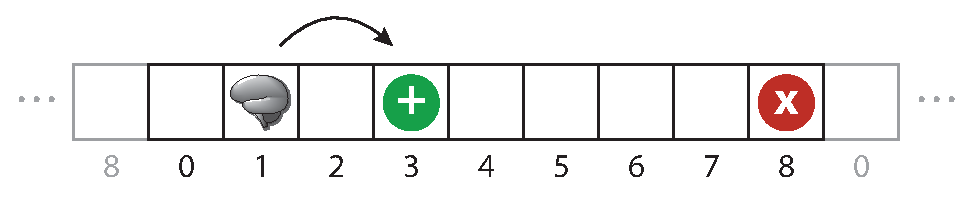
\includegraphics[height=2.5cm]{figs/grid_world_1D.eps}
\caption{The one-dimensional grid world.}
\label{grid_1D}
\end{figure}

As the name implies, this is a one-dimensional grid world. There are nine discrete states arrayed in a line, and the agent steps between them in increments of 1, 2, 3, or 4 steps in either direction. Stepping right from the rightmost state lands the agent in the leftmost state and vice versa, making the world into a ring. The fourth state from the left gives the agent a reward of 100 and the far right state inflicts a punishment (negative reward of -100). Every step the agent takes also incurs a cost of  1. This world was designed to be simple, yet non-trivial, and has proven very useful in troubleshooting \textsc{Becca}.

\subsection{\texttt{grid\_1D\_ms.py}}

The \texttt{ms} stands for `multi-step'. This world is identical to the \texttt{grid\_1D.py} world, except that the agent may only step in increments of one in either direction. Occasionally random perturbations place the agent in new positions and it must make its way back to its goal using multiple steps, rather than in a single step. This world requires multi-step planning and is a challenge for some learning agents. Right now \textsc{Becca} can only make its way directly back to the goal when it is within a couple of steps. It is waiting on better multi-step planning to perform really well on this task.

\subsection{\texttt{grid\_1D\_noise.py}}

The \texttt{noise} refers to the fact that the primitives reported by this world include a number of noise elements, whose values are randomly generated at each time step. It is similar to the  \texttt{grid\_1D.py} world, but has only three states.  The second of these gives a reward of 100, and the other two a punishment of -100. Many reinforcement learning algorithms do not have a mechanism for handling noise or irrelevant data and this world poses a challenge to them. 

\subsection{\texttt{grid\_2D.py}}

This is similar to \texttt{grid\_1D.py}, but extended to two dimensions, with 5 rows and 5 columns. Each dimension wraps around, similar to the one dimensional version. This gives the world a toroidal topology and makes it impossible to fall off of it or run into any walls. The agent can make steps of 1 or 2 columns or rows in any of the four compass directions. A location in the lower right portion of the world gives a reward of 100, and a second location in the upper left portion of the world gives a punishment of -100. And, as with the one dimensional world, every step incurs a cost of 1. The agent's position in the world is represented using an array of 25 primitives, one for each possible location. 

\begin{figure}
\centering
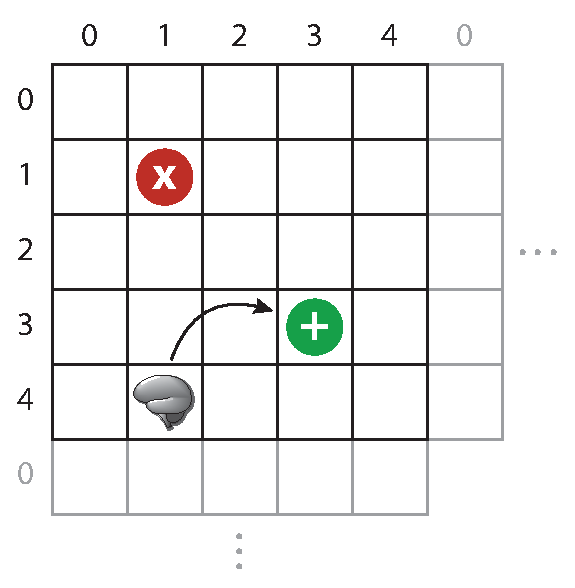
\includegraphics[height=10cm]{figs/grid_world_2D.eps}
\caption{The two-dimensional grid world.}
\label{grid_2D}
\end{figure}

\subsection{\texttt{grid\_2D\_dc.py}}

The \texttt{dc} stands for `decoupled' and refers to the fact that the column and row position of the agent are represented separately, each in an array of 5 primitive elements, giving this world a primitive array size of 10 rather than 25. This forces \textsc{Becca} to consider multiple inputs simultaneously when making decisions, making it a slightly more difficult world than \texttt{grid\_2D.py}.

\subsection{\texttt{image\_1D.py}}

The two major differences between the image worlds and the grid worlds are:

\begin{enumerate}
\item In the image worlds position is continuous, rather than discrete.
\item In the image worlds observations are arrays of sensors, rather than arrays of primitives.
\end{enumerate}

In the one dimensional case, the agent is looking at a mural (albeit a very boring one) and can shift its gaze right and left. It is rewarded for staring at the center of the mural.

The agent can move in increments of 1/4, 1/8, 1/16, and 1/32 of the mural width to both the right and left until it reaches the limits of the mural. All actions are also subject to an additional 10\% random noise. The agent's field of view is half as wide as the mural. The reward region is 1/16 as wide as the mural and positioned at its center. When the center of the agent's field of view falls within the reward region, the agent receives a reward of 100. Within its field of view, the agent averages pixel values in a 10 $\times$ 10 grid to create a coarsely pixelated version of the mural. Each coarse pixel can be between 0 (all black) and 1 (all white). The pixel values are passed through a center-surround filter, which calculates the extent to which each pixel value is lighter than or darker than its neighbors. The center-surround values are passed to the agent in a 100 element sensor array.

\begin{figure}
\centering
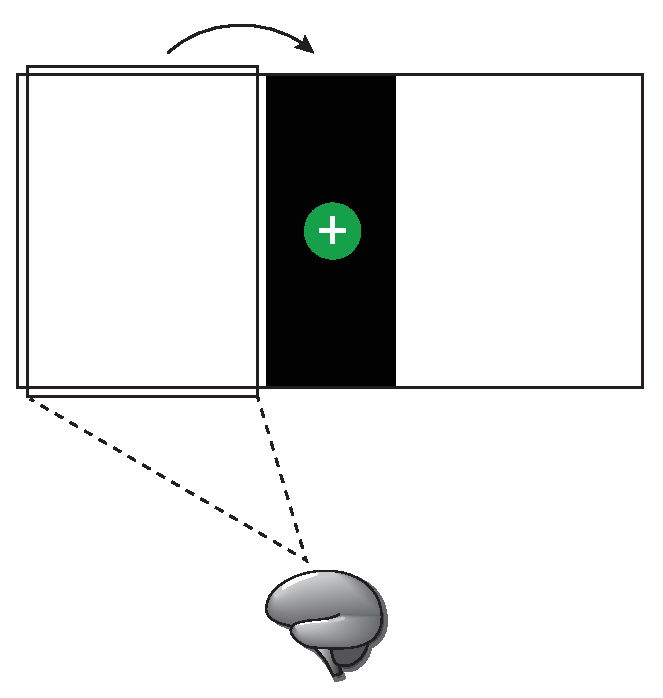
\includegraphics[height=8cm]{figs/image_world_1D.eps}
\caption{The one-dimensional image world.}
\label{image_1D}
\end{figure}

It's worth noting that a naive $\mathcal{Q}$-learning approach to this problem would require creating a $2^103$-element state table. The global information storage capacity is currently on the order of $2^70$ bytes.

\subsection{\texttt{image\_2D.py}}

This world is similar in many ways to the one dimensional version, just extended to a second dimension. In it, the agent must center its gaze both horizontally and vertically to receive the full reward. One difference is that it pixelizes its world into a 5 $\times$ 5 grid (resulting in a center-surround sensor array of 25 elements). A second difference is that the agent receives a reward of 50 if its gaze is centered horizontally and an additional reward of 50 if its gaze is centered vertically. 

\begin{figure}
\centering
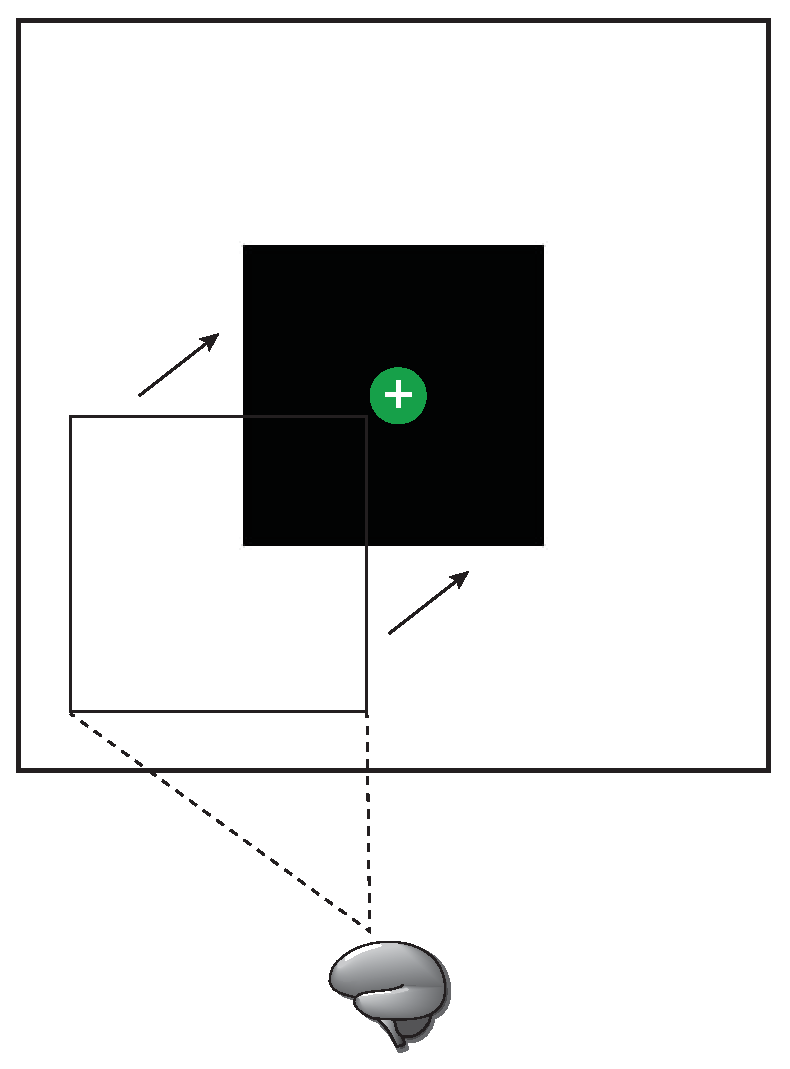
\includegraphics[height=12cm]{figs/image_world_2D.eps}
\caption{The two-dimensional image world.}
\label{image_2D}
\end{figure}


\subsection{\texttt{watch.py}}

The watch world is not part of the battery. It's a debugging tool. In it, the agent is exposed to image segments taken from a library of natural images, and it builds groups and feature representations from those image segments. It's helping to work out the kinks in the feature extraction heuristic, although I hope to integrate it into a task for future versions of the benchmark.


\subsection{\texttt{world\_utils.py}}

There are some jobs that crop up repeatedly in multiple worlds. This module is a common toolbox where functionality can be shared. So far this is limited to image processing functions, including center-difference filtering and visualizing features in image data.

